\chapter{Pruebas y resultados\label{sec:pruebasYResultados}}

En esta sección se presentan las pruebas principales a las que se ha sometido al sistema a lo largo del desarrollo, además de los resultados principales de cada una de ellas. Se divide la sección en dos partes. La primera, se centra en el primer prototipo, correspondiente al año académico 2013/2104, que fue utilizado satifactoriamente en una asignatura del Grado en Historia. La segunda parte se centra en el segundo (y actual) prototitpo, correspondiente al año académico 2014/2015, probado en una asignatura del Grado en Educación Infantil.

% IDEAS A VENDER:
% Generalizable y escalable. Podemos cambiar el modelo subyacente sin sufrir
% Meter el apartado de análisis de resultados
% Se han usado por 50 personas y ha aguantado
% Hablar de la base de datos. Del diseño y cómo se ha hecho
% Probado en entorno real

\section{2013/2014: Primer prototipo}

% Añadir la parte de análsis de datos

Durante el curso académico 2013/2014, 15 alumnos de la asignatura de ``Historia Antigua I'' del Grado en Historia de la Universidad Autónoma de Madrid utilizaron e-valUAM como herramienta de estudio y de evaluación. Fue el entorno donde se probó el primer prototipo, el cual ya permitía responder cuestionarios, pero no permitía a los profesores crearlos de forma autónoma ni les ofrecía posibilidades multimedia avanzadas (solo se permitía una imagen opcional por pregunta). De esta forma, la experiencia se centró en probar la experiencia de uso de los alumnos y la robustez del sistema para responder a los picos de demanda que sufre cuando se realiza un examen y todos los alumnos de una asignatura acceden simultáneamente.

\begin{figure}[htp!]
	\centering
	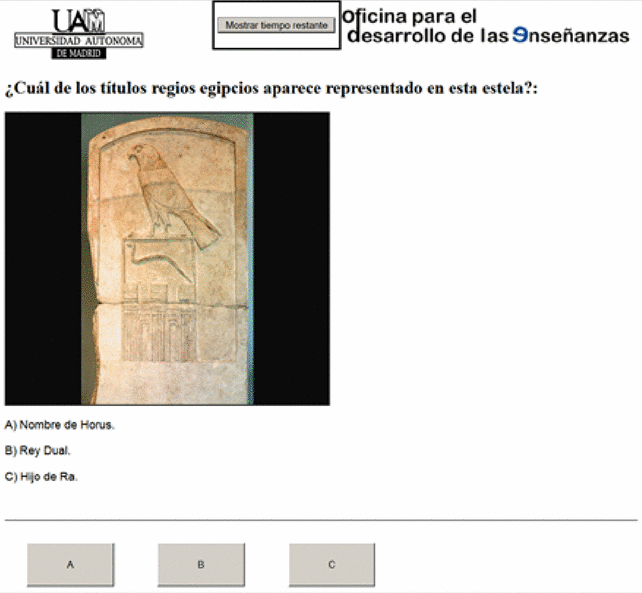
\includegraphics[width=0.75\textwidth,clip=true]{e-valUAM_primera_version}
	\caption{Interfaz del módulo del examen del primer prototipo}
	\label{fig:e-valUAM primera version}
\end{figure}

Desde el mes de octubre hasta el final del curso, los alumnos tuvieron disponibles 3 cuestionarios de autoevaluación y realizaron 4 exámenes. Los cuestionarios de autoevaluación estaban disponibles a los alumnos para que los realizarán tantas veces como quisieran. De los 15 alumnos, 6 utilizaron la aplicación para autoevaluación menos de 3 veces, mientras que otros 6 la utilizaron más de 15 veces. Los exámenes fueron dos parciales, un examen final para la convocatoria ordinaria y otro para la extraordinaria, al que solo se tuvieron que presentar 3 alumnos. La calificación determinada por la aplicación se ponderó en la nota final de la asignatura. A lo largo del año, entre tres profesores de Historia crearon un total de 372 preguntas, respondiéndose cada una de ellas 12,386 veces de media. 

Los resultados de la experiencia fueron muy satisfactorios. A nivel técnico, el sistema respondió como se esperaba durante todo el proceso, sin sufrir ningún tipo de caída. La mayor prueba de estrés del sistema fue el día del examen final. En las tres horas previas al examen se realizaron 31 accesos a los cuestionarios de autoevaluación, lo que supuso aproximadamente unas 300 peticiones al servidor. Cuando empezó el examen, los 15 alumnos lo realizaron a la vez, lo que supuso aproximadamente 68 peticiones por minuto al servidor durante los 20 minutos que duró el examen. El sistema logró almacenar todas las respuestas correctamente, seleccionar todas las preguntas siguientes siguiendo el modelo y ningún alumno tuvo que esperar entre preguntas ni sufrió ningún corte del servicio. Tampoco se registró ningún problema en los 3 meses que los alumnos hicieron un uso más intensivo del mismo (de noviembre de 2013 a enero de 2014).

% Hablar de qué se decidió cambiar
La experiencia de los alumnos con el sistema fue en general satisfactoria, aunque algunos mostraron malestar con el modelo del examen. Las mayores molestias venían provocadas porque no se pudieran dejar preguntas en blanco ni que se pudiera revisar una respuesta anterior. Aunque la segunda es una imposición del modelo (al depender las nuevas preguntas de las respuestas anteriores, estas no pueden cambiar), la primera sí se tuvo en consideración añadiendo la opción al modelo de la respuesta con duda.

De cara a la creación del segundo prototipo, además de añadir la respuesta con duda, se decidió crear el apartado de gestión del profesor, además de aumentar las capacidades de la aplicación para trabajar con ficheros multimedia. Así mismo, se hizo una actualización de la interfaz para incorporar un diseño responsive a la vez que se adaptadaba a todas las nuevas posibilidades multimedia que iban a incorporarse.

\section{2014/2015: Segundo prototipo}

Durante el curso académico 2014/2015, e-valUAM se utilizó en la asignatura de ``El Entorno como Instrumento Educativo'' del Grado en Educación Infantil. Las pruebas realizadas en este entorno fueron mucho más meticulosas que en el curso anterior, por varios motivos. 

Primero, los alumnos eran más y por lo tanto la aplicación se enfrentó a mayores picos de demanda. Segundo, se añadió más funcionalidad tanto para los profesores como para los alumnos. Tercero, los docentes utilizaron la aplicación como asistencia en su labor, pero además utilizamos la aplicación para conocer el nivel de conocimientos informáticos del que disponían los alumnos y conocer así mejor a los usuarios que iban a probar el sistema.

En las siguientes secciones se detallan cómo fueron cada una de las experiencias.
% Contar aquí que cambiamos el modelo

\subsection{Test de conocimientos informáticos}

El objetivo de este test era triple. Buscábamos conocer cuál era el nivel de informática de los alumnos que después utilizarían el sistema en su asignatura, probar exhaustivamente las opción de respuesta con duda y, por último, crear un nuevo modelo de evaluación utilizando la diferencia entre el conocimiento de expertos y un grupo de control.

Se creó un examen de 60 preguntas divididas en dos niveles de relevancia, cada nivel con 30 preguntas. Cada pregunta tenía 4 opciones, siendo una de ellas siempre ``No lo sé''. Además, fue el primer examen donde se utilizó la opción de respuesta con duda. Por estas peculiaridades, el modelo descrito en \ref{sec:modelo adapatacion} se varió ligeramente. Todos los alumnos respondían primero a las 30 preguntas del primer nivel y después a las 30 del segundo nivel, sin importar las respuestas previas.

El cuestionario lo respondieron 49 alumnos del Grado en Educación Infantil, que fueron el grupo de control, y alumnos del Grado en Ingeniería Informática y el Doble Grado con Matemáticas, que actuaron como grupo con conocimiento experto. En concreto 9 alumnos del último curso y 25 de segundo curso.

Este cuestionario permitió conocer mejor a los futuros usuario, además de probar el segundo prototipo del sistema antes de volver a utilizarlo en una asignatura real. Se hizo una prueba de estrés cuando los 25 alumnos de segundo curso realizaron a la vez el cuestionario. De nuevo, el sistema no mostró ningún problema. También sirvió para comprobar la robustez del diseño de la aplicación, ya que las modificaciones en el modelo de adaptación solo involucraron realizar cambios menores en uno de los ficheros, lo que parece indicar que la modularización se diseño correctamente. Por último, los resultados obtenidos en las respuestas han servido como base a la creación de un nuevo de evaluación, que se implementará en un futuro en e-valUAM. Más información sobre el nuevo modelo se puede encontrar en \cite{Molins15}.

\subsection{Alumnos del Grado en Educación Infantil}

Los 49 alumnos de ``El Entorno como Instrumento Educativo'' utilizaron e-valUAM de tres formas distintas. Primero, tuvieron a su disposición un cuestionario para la autoevaluación. Segundo, parte de su clasificación final surgió en función de un examen realizado mediante la plataforma. Tercero, como parte de la asignatura tenían que presentar un proyecto pedagógico para niños de eduación infantil, que tuvieron que plasmar en un cuestionario de e-valUAM. 

Desde diciembre de 2014, los alumnos tuvieron disponible durante un mes un cuestionario de autoevaluación con 91 preguntas distintas, divididas en 4 niveles. Los alumnos realizaron el cuestionario 838 veces en total. 5 de los 50 alumnos no lo intentarón ni una sola vez, mientras que hubo X que lo utilizaron más de Y veces.

El 14 de enero de 2015, realizaron el examen final utilizando también e-valUAM. Los 50 alumnos acudieron a los laboratorios de la EPS para realizar el examen de X preguntas durante Y minutos. Se utilizaron parte de preguntas de autoevaluación, algunas sin alterar, otras modificando los datos. También se añadieron preguntas nuevas.

Este examen sirvió como nueva prueba de estrés del sistema. Durante X minutos, 49 alumnos accedieron en simultáneo, realizando de media unas Y peticiones por minuto al servidor. Como en todas las ocasiones anteriores, no hubo ningún problema con la aplicación y toda la información quedó correctamente guardada.

Después del examen, se dió una charla de 15 minutos a los alumnos para explicarles cómo debían utilizar la interfaz del profesor, la cual tuvieron que utilizar para entregar un trabajo que se les exigía en la asignatura. Durante las dos semanas siguientes, los alumnos crearon en total Z cuestionarios nuevos, lo que supuso X preguntas nuevas y Y ficheros multimedia subidos al servidor. 

Para resolver incidencias o dudas, se puso a disposición de los alumnos un correo electrónico de contacto. Escribieron en total X personas, con Y incidencias y Z peticiones de nueva funcionalidad. % Descripción de lo que se hizo con la información de los alumnos %

Finalmente, el profesor de la asignatura corrigió el trabajo accediendo a la sección de profesor y consultando directamente los cuestionarios que cada grupo de alumnos había confeccionado.

\section{Comparativa con otras soluciones}